% Dit werk is gelicenseerd onder de licentie Creative Commons Naamsvermelding-GelijkDelen 4.0 Internationaal. Ga naar http://creativecommons.org/licenses/by-sa/4.0/ om een kopie van de licentie te kunnen lezen.
\documentclass[t]{beamer}

%%%%%%%%%%%%%%%%%%%%%%%%%%%%%%
% Packages
%%%%%%%%%%%%%%%%%%%%%%%%%%%%%%

\usepackage[dutch]{babel}               % Voor nederlandstalige hyphenatie (woordsplitsing)
\uselanguage{dutch}
\languagepath{dutch}
\usepackage{url}                        % Om url's te verwerken
\usepackage{graphicx,subfigure}         % Om figuren te kunnen verwerken
\usepackage[utf8]{inputenc}             % Om niet ascii karakters rechtstreeks te kunnen typen
\usepackage{multicol}
\usepackage[absolute,overlay]{textpos}

%%%%%%%%%%%%%%%%%%%%%%%%%%%%%%
% Layout
%%%%%%%%%%%%%%%%%%%%%%%%%%%%%%
\usetheme{Frankfurt}
\usefonttheme[onlymath]{serif}
\setbeamertemplate{footline}[page number]
\AtBeginSection[]
{
  \begin{frame}
    \frametitle{Inhoud}
    \tableofcontents[currentsection]
  \end{frame}
}

\setbeamertemplate{navigation symbols}{}

%%%%%%%%%%%%%%%%%%%%%%%%%%%%%%
% Title
%%%%%%%%%%%%%%%%%%%%%%%%%%%%%%
\title{Inleiding tot Inkscape}
\author{Brecht Baeten\inst{1}}
\institute{
	\inst{1}%
  		e-mail: brecht.baeten@gmail.com
}
\date{\today}
%%%%%%%%%%%%%%%%%%%%%%%%%%%%%%
% Omgevingen
%%%%%%%%%%%%%%%%%%%%%%%%%%%%%%

\begin{document}
	\frame{\titlepage}
%%%%%%%%%%%%%%%%%%%%%%%%%%%%%%%%%%%%%%%%%%%%%%%%%%%%%%%%%%%%%%%%%%%%%%%%%%%%%%%%
	\section{Inleiding}
%%%%%%%%%%%%%%%%%%%%%%%%%%%%%%%%%%%%%%%%%%%%%%%%%%%%%%%%%%%%%%%%%%%%%%%%%%%%%%%%
	\begin{frame}
		\frametitle{Voorbeelden}
		%\center
    	%\includegraphics[height=0.7\textheight{fig/inleiding/building_neighbourhood_cfd}\\
	\end{frame}
%%%%%%%%%%%%%%%%%%%%%%%%%%%%%%%%%%%%%%%%%%%%%%%%%%%%%%%%%%%%%%%%%%%%%%%%%%%%%%%%
	\section{Vector graphics}
%%%%%%%%%%%%%%%%%%%%%%%%%%%%%%%%%%%%%%%%%%%%%%%%%%%%%%%%%%%%%%%%%%%%%%%%%%%%%%%%
	\begin{frame}
		\frametitle{Bitmap vs. Vector}
		\vspace{0.5cm}
		\begin{columns}
			\begin{column}[T]{0.5\textwidth}
				\includegraphics[width=\textwidth]{fig/logo_zoom_png}
				\vspace{0.5cm}
				.bmp, .png, .jpg,...
			\end{column}
			\begin{column}[T]{0.5\textwidth}
				\includegraphics[width=\textwidth]{fig/logo_zoom_pdf}
				\vspace{0.5cm}
				.svg, .eps, .cdr, .ai, .pdf,...
			\end{column}
		\end{columns}
	\end{frame}
%%%%%%%%%%%%%%%%%%%%%%%%%%%%%%%%%%%%%%%%%%%%%%%%%%%%%%%%%%%%%%%%%%%%%%%%%%%%%%%%
	\begin{frame}
		\frametitle{Scalable Vector Graphics}
		\begin{itemize}
			\item .svg
			\item W3C norm (zoals html, css, xml,...)
			\item "leesbare" bestanden
			\item "definitie" van de tekening
		\end{itemize}
		\vspace{0.5cm}
		\begin{center}
			\hfill 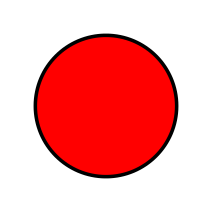
\includegraphics[width=0.2\textwidth]{fig/simpele_tekening}\\
			\vspace{-0.2cm}
			\includegraphics[width=\textwidth]{fig/simpele_tekening_bron.png}
		\end{center}	
	\end{frame}
%%%%%%%%%%%%%%%%%%%%%%%%%%%%%%%%%%%%%%%%%%%%%%%%%%%%%%%%%%%%%%%%%%%%%%%%%%%%%%%%
	\section{Inkscape}
%%%%%%%%%%%%%%%%%%%%%%%%%%%%%%%%%%%%%%%%%%%%%%%%%%%%%%%%%%%%%%%%%%%%%%%%%%%%%%%%
	\begin{frame}
		\frametitle{Werkbalken}
		\begin{center}
			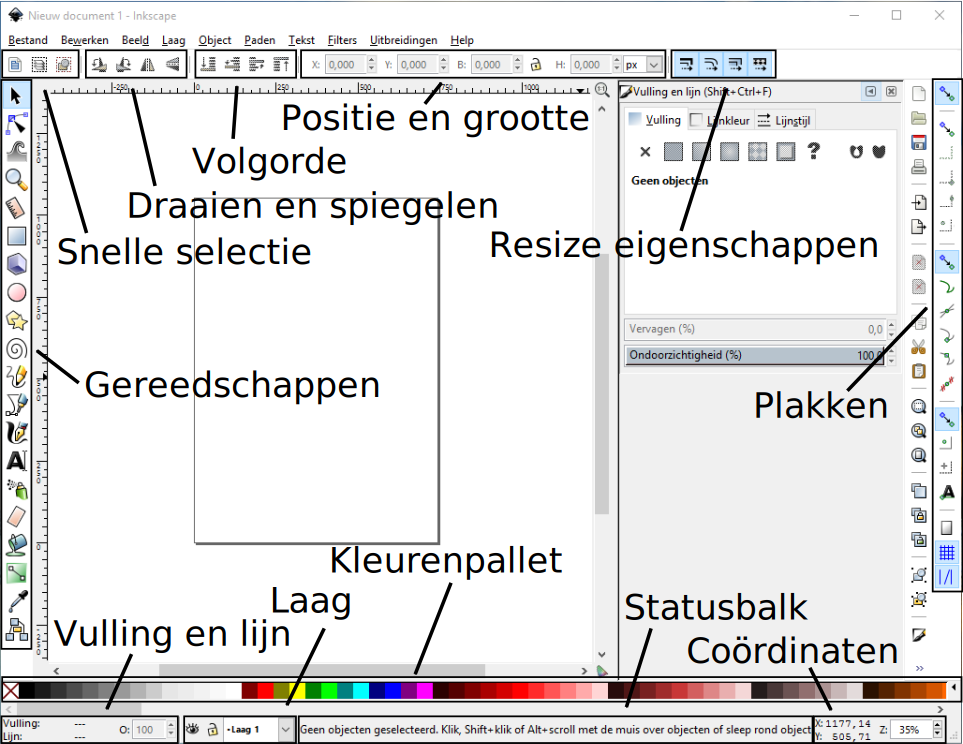
\includegraphics[height=0.85\textheight]{fig/inkscape_werkbalken}\\
		\end{center}	
	\end{frame}
%%%%%%%%%%%%%%%%%%%%%%%%%%%%%%%%%%%%%%%%%%%%%%%%%%%%%%%%%%%%%%%%%%%%%%%%%%%%%%%%
	\section{Objecten en Paden}
%%%%%%%%%%%%%%%%%%%%%%%%%%%%%%%%%%%%%%%%%%%%%%%%%%%%%%%%%%%%%%%%%%%%%%%%%%%%%%%%
	\begin{frame}
		\frametitle{Objecten}
		\begin{columns}
			\begin{column}[T]{0.6\textwidth}
				\begin{itemize}
					\item Rechthoek / 3D doos / Cirkel / Veelhoek / ster / Spiraal / Tekst
					\item Gereedschap selecterer en slepen
				\end{itemize}
				\begin{itemize}
					\item Vulling en lijn pallet openen via \emph{Object $>$ Vulling en lijn...}\\
					 of \textbf{Ctrl} + \textbf{Shift} + F\\
					 of dubbelklikken op vulling en lijn detail (links onderaan)
					\item Vulling, Lijnkleur, Lijnstijl
				\end{itemize}
			\end{column}
			\begin{column}[T]{0.4\textwidth}
				\includegraphics[height=0.8\textheight]{fig/inkscape_objecten}
			\end{column}
		\end{columns}
	\end{frame}
%%%%%%%%%%%%%%%%%%%%%%%%%%%%%%%%%%%%%%%%%%%%%%%%%%%%%%%%%%%%%%%%%%%%%%%%%%%%%%%%
	\begin{frame}
		\frametitle{Objecten en kleuren}
		\only<1>{
			\begin{center}
				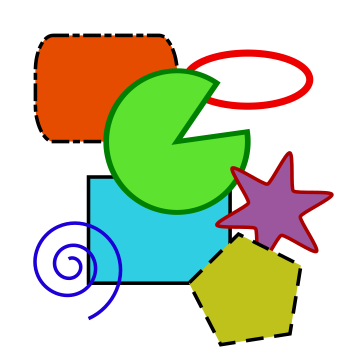
\includegraphics[height=0.8\textheight]{fig/objecten_en_kleuren}
			\end{center}
		}
		\only<2>{
			\textbf{Tips:}
			\begin{itemize}
				\item kleurenpallet klik = vulling kleur
				\item \textbf{Shift} + kleurenpallet klik  = rand kleur
			\end{itemize}
		}
	\end{frame}
%%%%%%%%%%%%%%%%%%%%%%%%%%%%%%%%%%%%%%%%%%%%%%%%%%%%%%%%%%%%%%%%%%%%%%%%%%%%%%%%
	\begin{frame}
		\frametitle{Objecten draaien en transformeren}
		\only<1>{
			\begin{columns}
				\begin{column}[T]{0.6\textwidth}
					\begin{itemize}
						\item Selectie gereedschap
						\item Vergroten / Verkleinen
						\item Draaien
						\item Scheeftrekken
						\item Verplaatsbaar referentiepunt
					\end{itemize}
					\begin{itemize}
						\item Ieder object heeft zijn eigen specifieke vervormings eigenschappen, beschikbaar via het object gereedschap
					\end{itemize}
				\end{column}
				\begin{column}[T]{0.4\textwidth}
					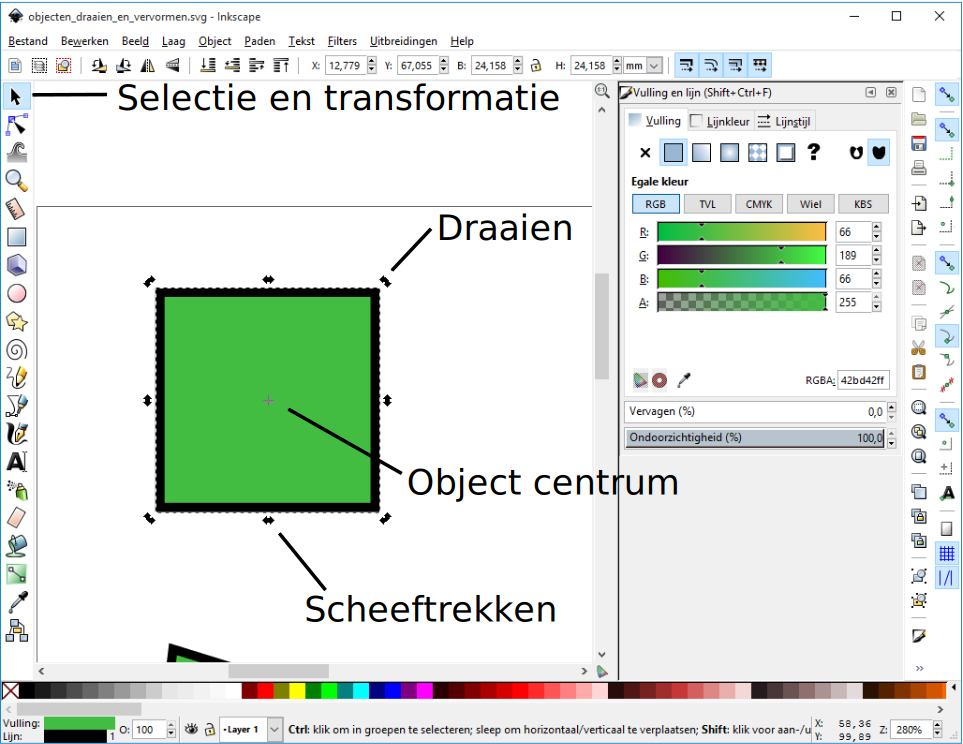
\includegraphics[height=0.8\textheight]{fig/inkscape_objecten_draaien_en_transformeren}
				\end{column}
			\end{columns}
		}
		\only<2>{
			\begin{center}
				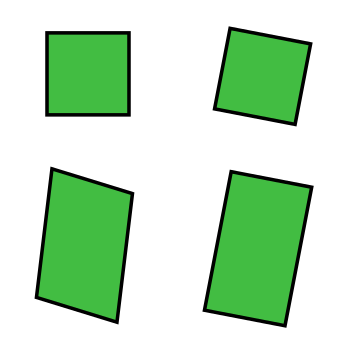
\includegraphics[height=0.8\textheight]{fig/objecten_draaien_en_transformeren}
			\end{center}	
		}
		\only<3>{
			\textbf{Tips:}
			\begin{itemize}
				\item \textbf{Ctrl} + vervormen = behoud van aspect ratio
				\item \textbf{Shift} + vervormen = schalen rond referentiepunt
				\item \textbf{Ctrl} + \textbf{Shift} + vervormen = combinatie van bovenstaande
				\item \textbf{Ctrl} + draaien = draaien met stappen van 15$^\circ$
				\item \textbf{Ctrl} + slepen = horizontaal of verticaal slepen
				\item slepen + \textbf{spatie} = object dupliceren en plaatsen
			\end{itemize}
		}
		
	\end{frame}
%%%%%%%%%%%%%%%%%%%%%%%%%%%%%%%%%%%%%%%%%%%%%%%%%%%%%%%%%%%%%%%%%%%%%%%%%%%%%%%%
	\begin{frame}
		\frametitle{Objecten vs. Paden}
		
		\vspace{-0.5cm}
		\hfill 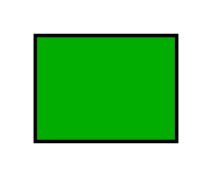
\includegraphics[width=0.2\textwidth]{fig/rechthoek_object}\\
		\vspace{-0.3cm}
		\includegraphics[height=2.5cm]{fig/rechthoek_object_bron.png}
		
		\hfill \includegraphics[width=0.2\textwidth]{fig/rechthoek_pad}\\
		\vspace{-0.3cm}
		\includegraphics[height=2.5cm]{fig/rechthoek_pad_bron.png}	
	\end{frame}
%%%%%%%%%%%%%%%%%%%%%%%%%%%%%%%%%%%%%%%%%%%%%%%%%%%%%%%%%%%%%%%%%%%%%%%%%%%%%%%%
	\begin{frame}
		\frametitle{Paden}	
		\only<1>{
			\begin{columns}
				\begin{column}[T]{0.6\textwidth}
					\begin{itemize}
						\item Losse hand tekenen
						\item Rechten / Bezier krommen / Splines
					\end{itemize}
					\begin{itemize}
						\item Van punt tot punt klikken voor een gebroken lijn
						\item Klikken en slepen voor een vloeiende lijn
						\item Dubbelklik om te eindigen
						\item Rechter muis klik om bij het vorige punt te stoppen
					\end{itemize}
				\end{column}
				\begin{column}[T]{0.4\textwidth}
					\includegraphics[height=0.8\textheight]{fig/inkscape_paden}
				\end{column}
			\end{columns}
		}
		\only<2>{
			\begin{columns}
				\begin{column}[T]{0.6\textwidth}
					\begin{itemize}
						\item Pad bewerken gereedschap
					\end{itemize}
					\begin{itemize}
						\item Nodes toevoegen / verwijderen
						\item Nodes samenvoegen / uiteen halen
						\item Nodes verbinden met een lijn
						\item Lijn tussen nodes verwijderen
					\end{itemize}
					\begin{itemize}
						\item Nodes slepen
						\item Node type (hoekig / glad / symmetrisch / auto)
						\item Node handvaten
					\end{itemize}
					\begin{itemize}
						\item Lijn vs. Curve
						\item Object naar pad
						\item Lijn (met dikte) naar pad
					\end{itemize}
				\end{column}
				\begin{column}[T]{0.4\textwidth}
					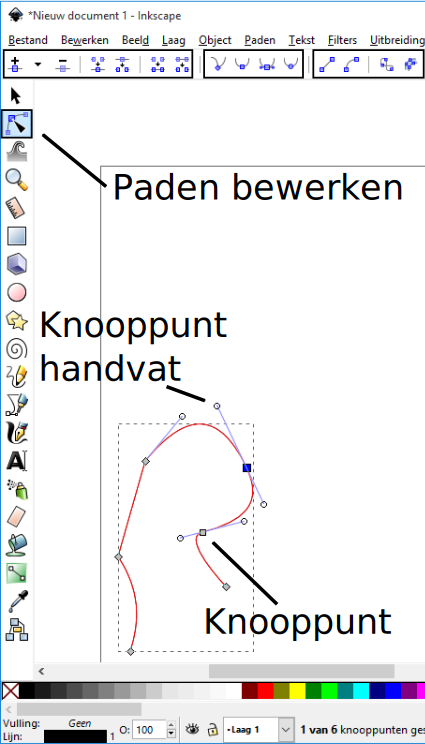
\includegraphics[height=0.8\textheight]{fig/inkscape_paden_bewerken}
				\end{column}
			\end{columns}
		}
		\only<3>{
			\begin{center}
				
\includegraphics[height=0.8\textheight]{fig/paden}
			\end{center}
		}
	\end{frame}
%%%%%%%%%%%%%%%%%%%%%%%%%%%%%%%%%%%%%%%%%%%%%%%%%%%%%%%%%%%%%%%%%%%%%%%%%%%%%%%%
	\begin{frame}
		\frametitle{Pad operaties}
		\only<1>{
			\begin{columns}
				\begin{column}[T]{0.6\textwidth}
					\begin{itemize}
						\item Elementaire bewerkingen op paden
					\end{itemize}
					\begin{itemize}
						\item Vereniging
						\item Verschil
						\item Overlap
						\item Uitsluiting
						\item Splitsing
						\item Snijden
					\end{itemize}
				\end{column}
				\begin{column}[T]{0.4\textwidth}
					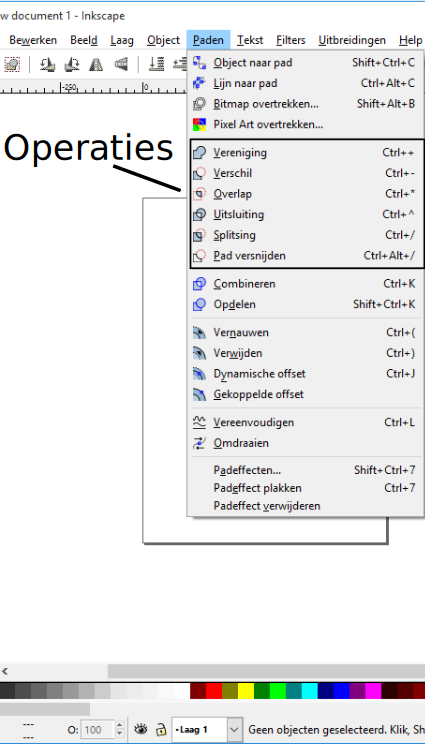
\includegraphics[height=0.8\textheight]{fig/inkscape_pad_operaties}
				\end{column}
			\end{columns}
		}
		\only<2>{
			\begin{center}
				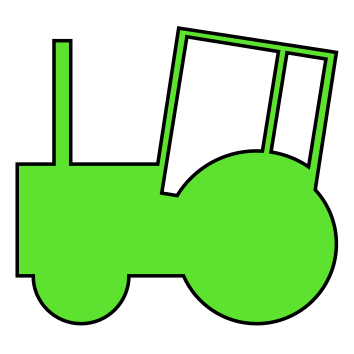
\includegraphics[height=0.8\textheight]{fig/pad_operaties}
			\end{center}
		}
	\end{frame}	
%%%%%%%%%%%%%%%%%%%%%%%%%%%%%%%%%%%%%%%%%%%%%%%%%%%%%%%%%%%%%%%%%%%%%%%%%%%%%%%%
	\section{Document eigenschappen}
%%%%%%%%%%%%%%%%%%%%%%%%%%%%%%%%%%%%%%%%%%%%%%%%%%%%%%%%%%%%%%%%%%%%%%%%%%%%%%%%



%%%%%%%%%%%%%%%%%%%%%%%%%%%%%%%%%%%%%%%%%%%%%%%%%%%%%%%%%%%%%%%%%%%%%%%%%%%%%%%%	
	\section{Templates}
%%%%%%%%%%%%%%%%%%%%%%%%%%%%%%%%%%%%%%%%%%%%%%%%%%%%%%%%%%%%%%%%%%%%%%%%%%%%%%%%



%%%%%%%%%%%%%%%%%%%%%%%%%%%%%%%%%%%%%%%%%%%%%%%%%%%%%%%%%%%%%%%%%%%%%%%%%%%%%%%%		
	\section{Afbeeldingen importeren}
%%%%%%%%%%%%%%%%%%%%%%%%%%%%%%%%%%%%%%%%%%%%%%%%%%%%%%%%%%%%%%%%%%%%%%%%%%%%%%%%	



%%%%%%%%%%%%%%%%%%%%%%%%%%%%%%%%%%%%%%%%%%%%%%%%%%%%%%%%%%%%%%%%%%%%%%%%%%%%%%%%	
	\section*{}
%%%%%%%%%%%%%%%%%%%%%%%%%%%%%%%%%%%%%%%%%%%%%%%%%%%%%%%%%%%%%%%%%%%%%%%%%%%%%%%%
	\begin{frame}
		\footnotesize
		\vspace{4cm}
		\includegraphics[height=0.3cm]{fig/cc} 
		\includegraphics[height=0.3cm]{fig/by} 
		\includegraphics[height=0.3cm]{fig/sa} 
		\quad \the\year\ Brecht Baeten
		\vspace{0.5cm}
		
    	Dit werk is gelicenseerd onder de licentie Creative Commons Naamsvermelding-GelijkDelen 4.0 Internationaal. Ga naar http://creativecommons.org/licenses/by-sa/4.0/ om een kopie van de licentie te kunnen lezen.
    	
    	\vspace{0.5cm}
    	De bron van dit document en alle tekeningen zijn beschikbaar op https://github.com/BrechtBa/inleiding-tot-inkscape
	\end{frame}	
	
\end{document}